\documentclass[border=4pt]{standalone}
\usepackage{tikz}
\usetikzlibrary{positioning, arrows.meta, calc, fit, backgrounds}
\usepackage{amsmath,amssymb}
\begin{document}
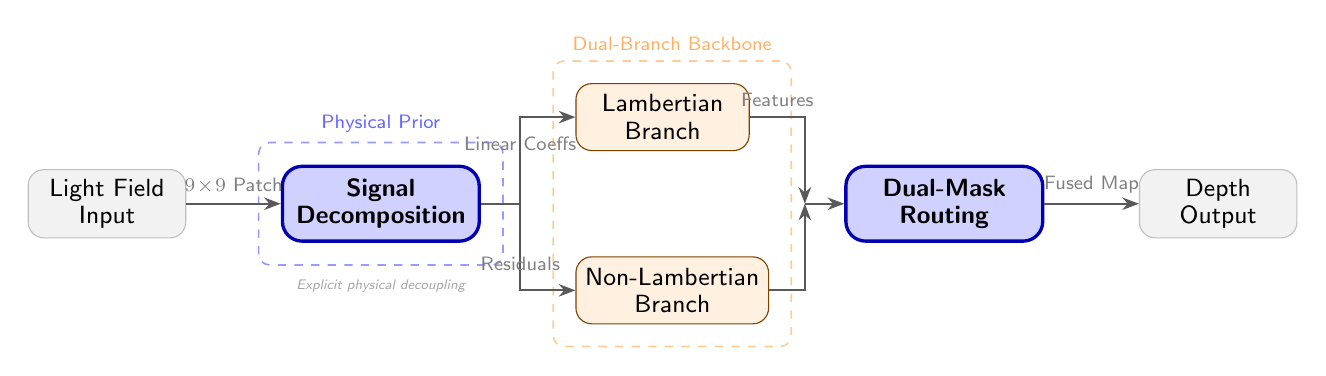
\begin{tikzpicture}[
  input/.style={draw, rounded corners=2mm, minimum width=2.0cm, minimum height=0.85cm,
                fill=gray!10, draw=gray!50, align=center, font=\sffamily\small},
  innov/.style={draw, rounded corners=2.5mm, minimum width=2.5cm, minimum height=0.95cm,
                fill=blue!18, draw=blue!70!black, line width=1.2pt, align=center,
                font=\sffamily\small\bfseries},
  proc/.style={draw, rounded corners=2mm, minimum width=2.2cm, minimum height=0.85cm,
               fill=orange!12, draw=orange!50!black, align=center, font=\sffamily\small},
  output/.style={draw, rounded corners=2mm, minimum width=2.0cm, minimum height=0.85cm,
                 fill=gray!10, draw=gray!50, align=center, font=\sffamily\small},
  arr/.style={-{Stealth[length=6pt]}, thick, color=black!65},
  gbox/.style={draw=#1, dashed, rounded corners=4pt, inner sep=8pt, line width=0.6pt},
  lbl/.style={font=\sffamily\scriptsize, text=black!50},
]

% --- Main nodes ---
\node[input]  (m1) {Light Field\\[-1pt]Input};

\node[innov, right=1.2cm of m1] (m2) {\textbf{Signal}\\[-1pt]\textbf{Decomposition}};

\node[proc, right=1.2cm of m2, yshift=1.1cm]  (m3) {Lambertian\\[-1pt]Branch};
\node[proc, right=1.2cm of m2, yshift=-1.1cm] (m4) {Non-Lambertian\\[-1pt]Branch};

\node[innov, right=1.2cm of m3, yshift=-1.1cm] (m5) {\textbf{Dual-Mask}\\[-1pt]\textbf{Routing}};

\node[output, right=1.2cm of m5] (m6) {Depth\\[-1pt]Output};

% --- Arrows: main flow ---
\draw[arr] (m1) -- node[lbl, above] {$9\!\times\!9$ Patch} (m2);

% Split from decomposition to branches
\draw[thick, color=black!65] (m2.east) -- ++(0.5,0) coordinate (split);
\draw[arr] (split) |- node[lbl, above, pos=0.25] {Linear Coeffs} (m3.west);
\draw[arr] (split) |- node[lbl, below, pos=0.25] {Residuals}     (m4.west);

% Merge from branches to dual-mask routing
\coordinate (merge) at ($(m5.west)+(-0.5,0)$);
\draw[arr] (m3.east) -| node[lbl, above, pos=0.25] {Features} (merge);
\draw[arr] (m4.east) -| (merge);
\draw[arr] (merge) -- (m5.west);

\draw[arr] (m5) -- node[lbl, above] {Fused Map} (m6);

% --- Group boxes (background) ---
\begin{scope}[on background layer]
  \node[gbox=blue!40, fit=(m2),
        label={[font=\sffamily\scriptsize, text=blue!60]above:Physical Prior}] (g1) {};
  \node[gbox=orange!40, fit=(m3)(m4),
        label={[font=\sffamily\scriptsize, text=orange!60]above:Dual-Branch Backbone}] (g2) {};
\end{scope}

% --- Annotation ---
\node[font=\sffamily\tiny\itshape, text=black!35, below=0.35cm of m2]
  {Explicit physical decoupling};

\end{tikzpicture}
\end{document}